% Diese Zeile bitte -nicht- aendern.
\documentclass[course=erap]{aspdoc}

%%%%%%%%%%%%%%%%%%%%%%%%%%%%%%%%%
%% TODO: Ersetzen Sie in den folgenden Zeilen die entsprechenden -Texte-
%% mit den richtigen Werten.
\newcommand{\theGroup}{230} % Beispiel: 42
\newcommand{\theNumber}{A204} % Beispiel: A123
\author{Vladislav Dzhorov \and Eslam Nasrallah \and Yiyang Xie}
\date{Sommersemester 2022} % Beispiel: Wintersemester 2019/20
%%%%%%%%%%%%%%%%%%%%%%%%%%%%%%%%%
% Diese Zeile bitte -nicht- aendern.
\title{Gruppe \theGroup{} -- Abgabe zu Aufgabe \theNumber}

\begin{document}
    \maketitle


    \section{Einleitung}\label{sec:einleitung}
    Das Ziel dieser Projektaufgabe ist ein Programm zum Dekomprimieren
    von BMP-Grafiken zu erstellen.
    Dafür muss man im Zuge der Projektaufgabe theoretisches Wissen aus der Mathematikum
    Anwendungszusammenhang verwenden und einen Algorithmus in C implementieren.
    \newline
    \newline
    Die Ursprünge der Datenkompression beruhen auf der Informationstheorie. \ \cite{shannon}
    \newline
    Im Wesentlichen bedeutet ``Kompression und Dekompression`` die Wahrscheinlichkeitsverteilung des Inhalts einer
    Datei zu ermitteln.
    Bei der Kompression wird die Redundanz beseitigt, bei der Dekompression wird die Redundanz wiederhergestellt.
    Es ist das Äquivalent dazu, denselben Inhalt in einer anderen Form auszudrücken.

%    \subsection{Information}\label{subsec:information}
%    Information besteht in der Unsicherheit, Veränderungen eines Signals vorhersagen zu können.
%    Der Informationsgehalt eines Zeichens $x\in\chi$ aus einem Alphabet $\chi$ hängt von der
%    Wahrscheinlichkeit $p(x)$ ab, dass das
%    informationstragende Signal zum Beobachtungszeitpunkt den diesem Zeichen zugeordneten Wert bzw.
%    Wertebereich annimmt.
%    Der Informationsgehalt $I$ des Zeichens $x$ mit der Auftrittswahrscheinlichkeit $p(x)$ ist definiert
%    als \ \cite{grnvsSlides}
%    \begin{center}
%        $ I(x) = -\log_{2}p(x) $  , mit $ [I] = $ bit.
%    \end{center}
%    Die Menge der Informationen ist umgekehrt proportional zur Wahrscheinlichkeit des Auftretens des Symbols.
%
%    \subsection{Informationsentropie}\label{subsec:informationsentropie}
%    Den mittleren Informationsgehalt einer Quelle bezeichnet man als Entropie \ \cite{grnvsSlides}
%    \begin{center}
%        $ H(X) = \sum_{x\in\chi}^{}p(x)I(x) = -\sum_{x\in\chi}^{}p(x)\log_2(p(x))$.
%    \end{center}
%    Die Informationsentropie und die damit zusammenhängenden Theoreme beschreiben den Grad der Redundanz in
%    mathematischer Hinsicht.
%    Mit Hilfe der Formel von Informationsentropie kann man den Grenzwert der Informationskodierung berechnen.

    \subsection{Analyse der Projektaufgaben}\label{subsec:analyse-der-projektaufgaben}
    Die Aufgabe des praktischen Teils des Projekts besteht darin, eine komprimierte Bitmap einzulesen und sie mit
    Hilfe des RLE-Algorithmus in eine unkomprimierte Bitmap umzuwandeln.
    \newline
    \newline
    Zu Beginn des Projekts wird ein Rahmenprogramm erstellt.
    Man soll darin C-I/O-Operationen implementieren, mit denen man eine BMP-Datei einlesen und einen Pointer auf diese
    Bilddaten und die zugehörigen Metadaten (z.B.\ Höhe und Breite) an die C-Funktion übergeben können.
    Anschließend sollte man eine neue BMP-Datei erstellen und die berechneten Werte nach dem Aufruf in diese schreiben.
    Das Ergebnis sollte mit dem üblichen Bildbetrachter lesbar sein.
    \newline
    \newline
    Die Hauptfunktion ist:
    \newline
    \newline
    $void$ \ bmp\_rld($const \ uint8\_t^*$ \ rle\_data, \ $size\_t$ \ len, \ $size\_t$ \ width, \ $size\_t$ \ height, \ $uint8\_t^*$ \ img)
    \begin{itemize}
        \item $const \ uint8\_t^* \ rle\_data:$ \ Dies ist das mit RLE komprimierte BMP-Bild, das der Benutzer dem
        Programm zur Verfügung stellt.
        \item $size\_t \ len:$ \ Zusätzlich wird der Benutzer die Länge von rle\_data angeben.
        Dies wirkt sich auf die Länge des Lesevorgangs und die Anzahl der Iterationen des Programms aus.
        \item $size\_t \ width,\ height:$ \ Die Breite und Höhe des Bildes, die sich auf die Größe und Auflösung des
        Bildes beziehen.
        Dies wirkt sich auf die Zuweisung von Speicherplatz durch das Programm aus.
        \item $uint8\_t^* \ img:$ \ Schließlich die Ausgabe des Programms.
        Abhängig von den oben genannten Parametern gibt das Programm ein dekomprimiertes BMP-Bild aus, das an dem Ort
        gespeichert wird, auf den dieser Zeiger zeigt.
        \noindent
    \end{itemize}


    \section{Lösungsansatz}\label{sec:losungsansatz}
    Im Folgenden werden die Konzepte und konkrete Implementierung des Bilddekompression Algorithmus tiefer betrachtet.
    \newline
    \newline
    Der Benutzer kann RLE-Daten in einem komprimierten BMP bereitstellen, wie es die Aufgabe erfordert.
    Die Größe der Daten beträgt 1Byte/8bit pro Einheit, weil das Programm nur das 8bpp-BMP-Format abdeckt.
    Wenn die Daten nicht in diesem erforderlichen Format vorliegen, kann das Programm die Datei nicht dekomprimieren.

    \subsection{Konzepte}\label{subsec:konzepte}
    Nach der Erläuterung der Projektaufgaben ist es wahrscheinlich, dass Personen, die nicht an dem Projekt
    teilgenommen haben, über einige Begriffe verwirrt sein werden.
    Daher ist es wichtig, die grundlegenden Konzepte zu verstehen, bevor wir den Lösungsansatz unserer Gruppe
    vorstellen.

    \subsubsection{Bitmap}\label{subsubsec:bitmap}
    Bitmap ist eine Form der Beschreibung eines Bildes in Form von computerlesbaren Daten.
    Windows Bitmap (BMP) ist das Standard Bilddateiformat für das
    Windows Betriebssystem und wird von einer Vielzahl von Windows Anwendungen unterstützt.
    Die Standard-Dateiendung für BMP-Bitmap-Dateien ist $.bmp$.
    Es besteht aus sogenannten Pixeln, denen jeweils eine Farbe zugeordnet ist.
    Diese Pixel können auf unterschiedliche Weise angeordnet werden, um verschiedene Muster zu bilden. \ \cite{imageProcessingInC}

    \subsubsection{Lauflängenkodierung}\label{subsubsec:lauflangenkodierung}
    Die Lauflängenkodierung bzw.
    RLE ist ein Algorithmus, der in Windows zur Kompression von Bilddateien verwendet wird.
    Windows unterstützt Formate zum Komprimieren von Bitmaps, die ihre Farben mit 8 oder 4 Bit pro Pixel
    definieren. \ \cite{rle}
    \newline
    \newline
    Gemäß den Anforderungen dieses Praktikums muss das Programm explizit nur das 8bpp-BMP-Format abdecken!
    \newline
    \newline
    Die Grundidee ist, dass benachbarte Pixel mit derselben Farbe in einer Scanzeile durch zwei Bytes
    dargestellt werden. \ \cite{bildkompressionSlides}
    Das erste Byte ist die Anzahl der Wiederholungen des Pixels, das Zweite ist der Wert oder die Farbe des Pixels,
    z.B\@.
    \begin{center}
        RRRRRRRRGGBBBBBB \ -----> \ 8R2G6B
    \end{center}
    \noindent Nach der RLE-Kompression ist die Länge der Zeichenfolge signifikant kürzer als vorher.

    \subsection{Allgemeiner Algorithmus}\label{subsec:allgemeiner-algorithmus}
    An dieser Stelle kann man davon ausgehen, dass man die Projektaufgabe, die Hauptfunktion, die Parameter
    und die Grundkonzepte verstanden hat.
    \newline
    \newline
    Der Algorithmus zur Bilddekompression funktioniert wie folgt. \ \cite{bitmapCompression}
    \begin{itemize}
        \item Alle 2 Bytes enthalten Informationen über eine Sequenz mit einer einzigen Farbe.
        \begin{itemize}
            \item[-] Das erste Byte ist die Anzahl der Wiederholungen des Pixels.
            \item[-] Das zweite Byte ist der Wert oder die Farbe des Pixels.
        \end{itemize}
        \item Wenn das erste Byte Null ist, wird das zweite Byte betrachtet.
        \begin{itemize}
            \item[-] Wenn es ebenfalls 0 ist, bedeutet dies das Ende der Zeile.
            \item[-] Wenn es eine 1 ist, bedeutet dies das Ende der Datei.
            \item[-] Wenn es eine 2 ist, bedeutet dies das Delta.
            \item[-] Die 2 Bytes nach dem Escape enthalten vorzeichenlose Werte, die den Versatz nach rechts und nach
            oben des nächsten Pixels von der aktuellen Position angeben, z.B\@.
            \newline
            Die Bedeutung von [00 02 05 01] ist, dass der aktuelle Zeiger 5 Byte nach rechts und dann eine Zeile nach
            unten geschoben wird, d.h.\ ein Teil der Pixel wird übersprungen.
        \end{itemize}

        \item Zum Schluss werden die dekodierten Daten im $uint8\_t^* \ img$ gespeichert.
    \end{itemize}
    \noindent Hinweis: RLE-Daten verwenden eine spezielle Struktur, um mehrere, sich nicht wiederholende
    Datenpixel zu speichern, z.B\@.
    \begin{itemize}
        \item $[00 \ 03 \ 45 \ 56 \ 67 \ 00]$ dekomprimiert zu $[45 \ 56 \ 67]$.
        \item $[00 \ 04 \ 39 \ 56 \ 67 \ 12]$ dekomprimiert zu $[39 \ 56 \ 67 \ 12]$.
        \noindent
    \end{itemize}
    \noindent d.h.\ das erste Byte ist die Kennung ``00``.
    Das zweite Byte hat einen Wert größer als 2, der die Länge der sich nicht wiederholenden Pixeldaten
    angibt (Zeile 5) \ \cite{bitmapCompression}.
    Jedes nachfolgende Byte sind die spezifischen Pixeldaten.
    \newline
    \newline
    Wenn das zweite Byte eine gerade Zahl ist, ist die Struktur wie oben beschrieben.
    \newline
    Wenn das zweite Byte eine ungerade Zahl ist, wird am Ende dieser Dateneinheit eine zusätzliche ``00`` angefügt.

    \begin{figure}[htbp]
        \begin{minipage}[t]{0.48\textwidth}
            \centering
            
\includegraphics[height=3cm, width=3cm]{diagram/Lenna_mistake0}
            \caption{Fehlerbeispiel}
        \end{minipage}
        \begin{minipage}[t]{0.48\textwidth}
            \centering
            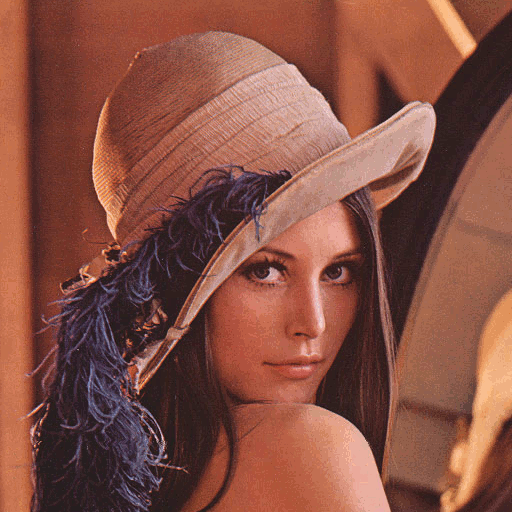
\includegraphics[height=3cm, width=3cm]{diagram/Lenna_original}
            \caption{Korrekte Ausgabe}
        \end{minipage}\label{fig:figure2}
        \newline
        (Nur repräsentative Beispiele, weitere Tests finden sich in der praktischen Abteilung.)
    \end{figure}
    \noindent Das Ignorieren von Farben, die sich nicht wiederholen, führt nach der Dekompression zu einem erheblichen
    Datenverlust.

    \subsection{Implementierung in C}\label{subsec:implementierung-in-c}
    Ausgehend von der Struktur der RLE-Daten kann man sich intuitiv vorstellen, eine Schleife zum Lesen und
    Verarbeiten der Daten zu verwenden.
    Die Anzahl der Iterationen wird durch die Länge der RLE-Daten begrenzt, d.h.\ durch den Parameter $size\_t \ len$.
    Die Schleife liest die Daten der Größe 2 Bytes und schreibt dann das Ergebnis in einer verschachtelten Schleife
    an die Stelle, auf die $uint8\_t^* \ img$ zeigt.
    \newline
    \newline
    Der abgekürzte Code lautet wie folgt, der vollständige Code ist in $bmp\_rld\_c\_basic$ in
    der Datei \ $main.c$.
    \lstset{language=C}
    \begin{lstlisting}
void bmp_rld_c_basic(const uint8_t *rle_data, size_t len, size_t width, size_t height, uint8_t *img) {
    ...     // initialization

    for (size_t i = 0; i < len;) {
        if (rle_data[i] == 0 && rle_data[i + 1] > 2) {
            ...     // non-repeating colors
        } else if (rle_data[i] == 0 && rle_data[i + 1] == 0) {
            ...     // end of line
        } else if (rle_data[i] == 0 && rle_data[i + 1] == 1) {
            ...     // end of bitmap
        } else if (rle_data[i] == 0 && rle_data[i + 1] == 2) {
            ...     // delta marker
        } else {
            ...     // normal decoding with loop
            for (; j < limit; j++) {
                ...     //copy pixels byte by byte
            }
        }
    }
}

    \end{lstlisting}
    \noindent Der Vorteil dieser Implementierung in C ist, dass der Code logisch
    verständlich, mit guter Lesbarkeit ist und schnell implementiert werden kann.

    \subsection{Implementierung in Assembler x86-64}\label{subsec:implementierung-in-assembler-x86-64}
    Diese Implementierung folgt der obigen C-Implementierung.
    Das Rahmenprogramm ist in C geschrieben und die Bilderdekompression-Funktion ist in Assembler implementiert.
    \newline
    \newline
    Der vollständige Code befindet sich in der Datei $bmp.S$.

    \subsection{Implementierung in Assembler x86-64 mit SIMD}\label{subsec:implementierung-in-assembler-x86-64-mit-simd}
    Bei der SIMD-Implementierung werden 16 Pixels gleichzeitig verarbeitet.
    Das Verfahren ähnelt der SISD-Implementierung, aber die Effizienz wird verbessert.
    \newline
    \newline
    Der Code verwendet SIMD an zwei Stellen.
    \begin{enumerate}
        \item Wenn mindestens 16 Bytes der gleichen Farbe hintereinander auftreten, werden 16 Bytes auf einmal
        in die Ausgabe geschrieben.
        \item Wenn mindestens 16 Byte nicht wiederkehrender Farben in einer Reihe vorhanden sind, werden 16 Byte
        gleichzeitig gelesen und in die Ausgabe geschrieben.
    \end{enumerate}
    \noindent Der Vorteil dieser iterativen SIMD-Implementierung besteht darin, dass sie die Vorteile des ursprünglichen Codes
    beibehält und gleichzeitig eine höhere Dekompressionseffizienz für Bilder mit mehreren Farbwiederholungen aufweist.
    \newline
    \newline
    Der vollständige Code befindet sich in der Datei $bmpOpt.S$.

    \subsection{Implementierung in C mit SIMD-Idee}\label{subsec:implementierung-in-c-mit-simd-idee}
    Ursprünglich wurde eine Erweiterung von SSE, d.h.\ Intel Intrinsics, verwendet.
    Nach einigen Experimenten haben wir festgestellt, dass eine Implementierung unter Verwendung der
    Funktionen \ $memset$ \ und \ $memcpy$, welche in der Bibliothek \ $string.h$ \ sind, wesentlich
    schnellere Laufzeiten liefert.
    \newline
    Deshalb werden die Intel Intrinsics SSE-Befehle in unserem Code dadurch ersetzt.
    \newline
    \newline
    Im Allgemeinen folgt diese Implementierung noch dem Abschnitt 2.6 Implementierung in Assembler x86-64 mit SIMD,
    allerdings mit geänderten Implementierungsdetails.
    \newline
    \newline
    Der vollständige Code findet sich in $bmp\_rld\_C\_opt$ in der Datei \ $main.c$.


% TODO: Je nach Aufgabenstellung einen der Begriffe wählen


    \section{Korrektheit}\label{sec:korrektheit}
    In diesem Projekt soll ``Korrektheit`` ausgewählt wird,
    da RLE ein verlustfreier Kompressionsalgorithmus ist.
    Die Dekompression erfolgt nach denselben Regeln wie die Kompression und die wiederhergestellten Daten sind mit
    den vorkomprimierten Daten identisch, nicht nur ähnlich, so dass ``Genauigkeit`` hierfür eindeutig nicht ausreicht.
    \newline
    \newline
    Um die Korrektheit zu überprüfen, werden Bilder mit den verschiedenen Implementierungen dekomprimiert und mit dem
    Originalbild verglichen.

    \subsection{Testcases}\label{subsec:testcases}
    Zunächst wurde versucht, im Internet nach Bitmaps zu suchen, die mit der RLE-Kodierung komprimiert wurden, sowie
    die Originalbilder.
    Es konnten allerdings keine Testfälle im Bitmap-Format gefunden werden, sondern ausschließlich im JPEG-Format,
    welches weniger Speicherplatz benötigt und für die Übertragung im Netz besser geeignet ist.
    \newline
    \newline
    Anschließend wurden die Originalbilder mit Hilfe der Online-Kompression im Internet automatisch komprimiert, aber
    die Online-Kompression war nicht die verlustfreie Kompression, die für die Aufgabe erforderlich war, oder es wurde
    keine RLE-Kodierung verwendet.
    \newline
    \newline
    Nach Diskussionen und Experimenten wurde schließlich Photoshop $v23.4.1$ verwendet \ \cite{bmpExtension}, um
    manuell Bilder zu erstellen.
    \newline
    \newline
    Am Anfang wird sichergestellt, dass der Typ des von Photoshop erzeugten Ergebnisses ``Bitmap`` ist.
    Ist dies der Fall, werden die Daten im Header byteweise verglichen, da die Informationen über die Breite, Höhe und
    Größe des Bildes aus dem Header ausgelesen werden können.
    Anschließend werden diese Daten, die sogenannte Pixelanordnung, byteweise verglichen. \ \cite{bitmapStorage}

    \subsection{Fehlerbeispiel}\label{subsec:fehlerbeispiel}
    Zunächst lieferte die ursprüngliche Lösungsansatz nicht perfekte Ergebnisse.
    Das Bild wurde insgesamt wiederhergestellt, aber es ist offensichtlich, dass es Pixelverschiebungen im Bild gibt.

    \begin{figure}[htbp]
        \begin{minipage}[t]{0.48\textwidth}
            \centering
            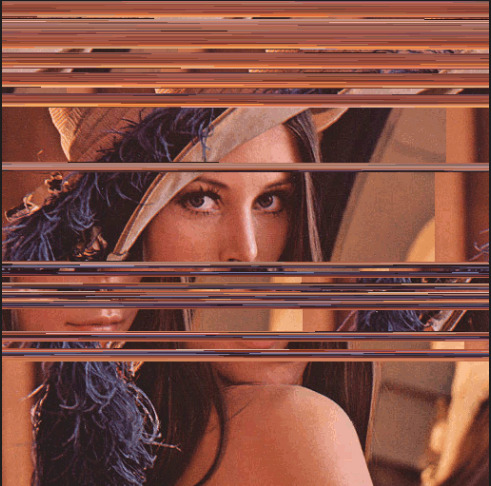
\includegraphics[height=3cm, width=3cm]{diagram/Lenna_mistake1}
            \caption{Fehlerbeispiel}
        \end{minipage}
        \begin{minipage}[t]{0.48\textwidth}
            \centering
            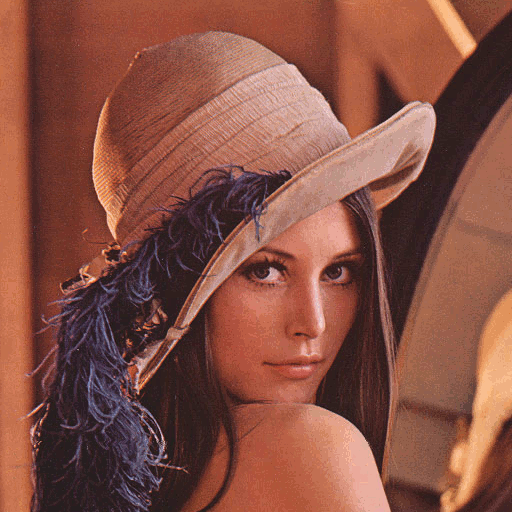
\includegraphics[height=3cm, width=3cm]{diagram/Lenna_original}
            \caption{Korrekte Ausgabe}
        \end{minipage}\label{fig:figure}
        (Nur repräsentative Beispiele, weitere Tests finden sich in der praktischen Abteilung.)
    \end{figure}
    \noindent Die folgenden Aspekte müssen berücksichtigt werden,
    um die Korrektheit der Lösungsansatz zu gewährleisten.

    \subsection{Behandlung spezieller Marker}\label{subsec:behandlung-spezieller-marker}
    Es gibt Bytes in den RLE-Daten, die nicht farbbezogen sind oder die Standardfarbe darstellen.
    Diese Datensegmente können nicht einfach ignoriert werden,
    d.h.\ der Speicherplatz für diese Bytes sollte reserviert und vollständig durch $0x00$ ersetzt werden.
    Andernfalls haben die Daten einen unerwarteten Offset.
    \newline
    \newline
    Standardmäßig werden die Pixel mit einem Wert von 0 die am häufigsten auftritten Farben im Bild darstellen.
    Es ist effizienter, diesen Pixeln durch den Delta-Marker, Zeilenvorschub-Marker oder End-Marker direkt
    den Wert 0 anzuweisen.

    \subsection{Behandlung von Byte Alignment}\label{subsec:behandlung-von-byte-alignment}
    Das Bitmap-Format legt fest, dass die Anzahl der Bytes, die eine gescannte Zeile belegt, ein Vielfaches von 4 sein
    muss.
    \newline
    \newline
    Andernfalls wird es mit Nullen aufgefüllt\cite{bitmapPadding},
    d.h.\ diese mit Photoshop erzeugten Bilder enthalten immer 0--3 Bytes Padding am Ende der Datei, z.B\@.
    \newline
    \newline
    im 8bpp-BMP-Format
    \begin{itemize}
        \item \ $width = 5$, jede Zeile belegt 5 Bytes, am Ende von $buf$ wird mit 3 $0x00$ gefüllt
        \item \ $width = 6$, jede Zeile belegt 6 Bytes, am Ende von $buf$ wird mit 2 $0x00$ gefüllt
        \item \ $width = 7$, jede Zeile belegt 7 Bytes, am Ende von $buf$ wird mit 1 $0x00$ gefüllt
    \end{itemize}

    \subsection{Konkrete Behandlungen}\label{subsec:konkrete-behandlungen}
    Für die Behandlung spezieller Marker werden zusätzliche Variablen
    $uint8\_t \ pass$ und $uint8\_t \ linecounter$ deklariert.
    \newline
    \newline
    Nach der Verarbeitung der Pixel wird der Wert von $linecounter$ aktualisiert.
    Schließlich wird die Anzahl der 0-Werte am Ende jeder Zeile damit ausgerechnet.
    \begin{center}
        $pass = width - linecounter;$
    \end{center}
    \noindent Für die Behandlung von Byte Alignment werden die zusätzliche Variable
    \begin{center}
        $uint8\_t \ linePadd = (4 - width \ \% \ 4) \ \% \ 4;$
    \end{center}
    deklariert.
    $linePadd$ bestimmt die Anzahl der Paddings, die die Byte-Alignment erforderlich sind.
    \newline
    \newline
    Insbesondere für den Delta-Marker wird die Gesamtzahl der Paddings damit ausgerechnet.
    \begin{center}
        $pass = up * width + right + linePadd * up;$
    \end{center}


    \section{Performanzanalyse}\label{sec:performanzanalyse}
    Hinweis: Nicht jede Implementierung ist effizient und manchmal kann sich die Performanz sogar verschlechtern.

    \subsection{Allgemeine Information}\label{subsec:allgemeine-information}
    Das verwendete System hat folgende Spezifikationen: Intel(R) Core(TM) i7-10750H CPU, 2.60 GHz, 16 GB
    Arbeitsspeicher, Ubuntu 18.04.6 LTS, 64 bit, Linux Kernel 5.4.0-122-generic.
    Kompiliert wurde mit GCC 7.5.0 mit der Option -O2.
    \newline
    \newline
    Um die Unterschiede deutlich darzustellen, wurden die Laufzeiten mit verschiedenen RLE-komprimierten
    Bildern berechnet.
    Die ausgewählten Eingabebilder sind repräsentativ und daher ausreichend, um die Performanz jeder Implementierung
    zu bestimmen.

    \begin{enumerate}
        \item Lena ----- wird von dem Projekt zur Verfügung gestellt und ist ein klassischer
        Anwendungsfall im Bereich der Bildverarbeitung.
        ``Lena`` hat relativ unregelmäßige Farben.
        Die Pixelwiederholungen sind gering.
        \item Pinktrees ----- ist ähnlich wie ``Lena``, aber es ist etwa 3 Mal größer als das erste.
        \item Black white ----- hat relativ homogene Farben und eine große Anzahl von
        sich wiederholenden Pixelblöcken.
        \item Black hole ----- ist ähnlich wie ``Black white``, aber seine Dateigröße ist viel
        größer als die der ersten drei, ca.\ 20 Mal größer, d.h.\ das zweite Bild hat eine
        höhere Auflösung.
        \noindent
    \end{enumerate}
    \noindent Die Berechnungen wurden jeweils 5-mal durchgeführt.
    Das arithmetische Mittel jeder Eingabegröße wurde in den Grafiken eingetragen.

    \subsection{Ergebnisse}\label{subsec:ergebnisse}
    Die Analyse wird auf der Steuerungsvariable basieren, d.h.\ dass die Effizienz verschiedener Implementierungen mit
    derselben Eingabe verglichen wird.

    \subsubsection{Datenmenge vor und nach der Dekompression}\label{subsubsec:datenmenge-vor-und-nach-der-dekompression}

    \begin{figure}[htbp]
        \begin{minipage}[t]{\textwidth}
            \centering
            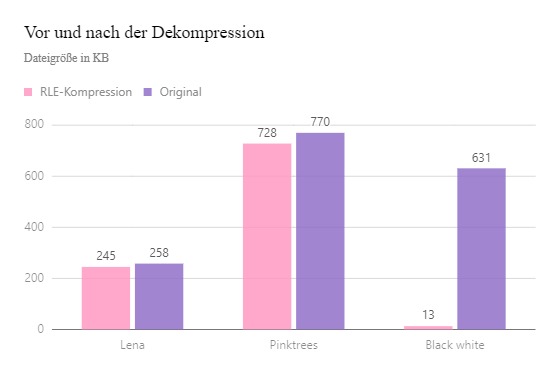
\includegraphics[height=6cm, width=10cm]{diagram/filesize}
        \end{minipage}\label{fig:figure4}
        Die getesteten Bilder befinden sich im Ordner $TestImages$, nicht im $Ausarbeitung/diagram$.
        \noindent
    \end{figure}
    \noindent ``Black white`` hat die relativ homogenen Farben, z.B.\ zahlreiche schwarze oder weiße Pixel.
    Die wiederholenden Pixelblöcken können erheblich auf nur 2 Bytes komprimiert werden, deswegen hat es einen großen
    Unterschied in der Dateigröße vor und nach der Kompression.
    \newline
    \newline
    Im Gegensatz dazu haben Bilder wie ``Lena`` and ``Pinktrees``, die mit wenigen Farbwiederholungen sind, eine sehr
    geringe Kompressionsrate.
    Im Extremfall kann die Datenmenge durch die RLE-Kompression sogar noch größer werden.
    \newline
    \newline
    Daraus wird geschlossen, dass die Höhe der RLE-Kompressionsrate abhängig weitgehend von den
    Eigenschaften des Bildes selbst ist.
    Je größer der Bildblock mit der gleichen Farbe, desto höher ist die erzielte Kompressionsrate.

    \subsubsection{Laufzeitvergleich zwischen Implementierungen}\label{subsubsec:laufzeitvergleich-zwischen-implementierungen}

    \begin{figure}[htbp]
        \begin{minipage}[t]{\textwidth}
            \centering
            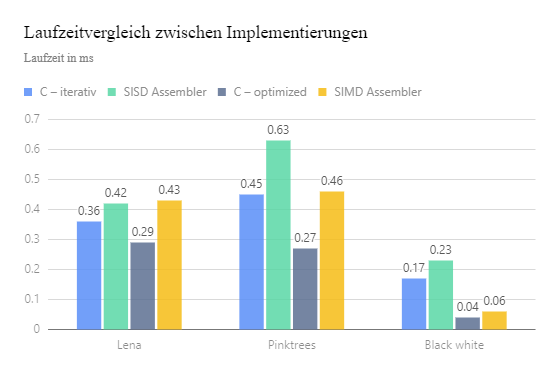
\includegraphics[height=6cm, width=10cm]{diagram/togather_time}
        \end{minipage}\label{fig:figure6}
        \noindent
    \end{figure}
    \noindent Aus den Grafiken geht hervor, dass der C-Code aufgrund der Verwendung von O2 bei der Kompilierung sogar
    effizienter als der Assembler-Code ist.
    Compiler Optimierungsstufe 2 kombiniert die Optimierungen von O1 und viele andere Optimierungen,
    z.B\@.
    \begin{itemize}
        \item \ $-fgcse$, um Redundanzen zu vermeiden
        \item \ $-fstrength-reduce$ und $-frerun-cse-after-loop$ entfernen die von der Schleife
        erzeugten Variablen und zerlegen sie
        \item \ $-fcse-follow-jumps$ optimiert Sprunganweisungen, z.B.\ if-else-Anweisungen
    \end{itemize}
    \noindent Darüber hinaus ist der optimierte C-Code effizienter, insbesondere im Fall der Eingaben ``Black white``.
    Das liegt daran, dass ``Black white`` die meisten Farbwiederholungen aufweist.
    \newline
    \newline
    Im Vergleich zu unserer Assembler-SIMD Implementierung ist die optimierte C Implementierung aufgrund der
    Verwendung von \ $memset$ \ und \ $memcpy$ \ wesentlich schneller.
    Wenn man den Code von \ $bmp\_rld\_C\_opt$ \ disassembliert, kann man sehen, dass diese beide Funktionen
    SIMD-Instruktionen zusammen mit anderen Optimierungen wie ausgerichtete Speicherzugriffe, Prefetching,
    ``Loop unrolling`` und auch CPU-spezifische Optimierungen verwenden.
    \newline
    \newline
    Daraus lassen sich zwei Schlüsse ziehen:
    \begin{enumerate}
        \item \ $memset$ \ und \ $memcpy$ \ sind für diese Aufgabe sehr gut geeignet,
        da eine große Menge an wiederholenden Daten kopiert werden muss.
        \item Die Laufzeit der Dekompression nach der Optimierung ist umgekehrt proportional zur
        Menge an wiederholenden Daten.
    \end{enumerate}
    \noindent Dies entspricht auch der Formel für die Informationsentropie: \ \cite{grnvsSlides}
    \begin{center}
        $ H(X) = \sum_{x\in\chi}^{}p(x)I(x) = -\sum_{x\in\chi}^{}p(x)\log_2(p(x))$.
    \end{center}
    \noindent Je höher die Wahrscheinlichkeit des Auftretens eines Symbols ist, desto weniger gültige Informationen repräsentiert
    es und desto weniger Verbrauch Dekompression benötigt.

    \subsubsection{Allgemeiner Laufzeitvergleich}\label{subsubsec:allgemeiner-laufzeitvergleich}

    Der allgemeine Vergleich zeigt, dass ``Black hole`` viel längere Zeit als ``Lena`` für die
    Dekompression braucht.
    Diese wird durch die Größe des Bildes, sogenannte Auflösung, bestimmt.
    \begin{itemize}
        \item Die Laufzeit des optimierten C für ``Black hole`` beträgt 1,02ns und für ``Lena`` 0,29ns.
        \item Die Dateigröße für ``Black Hole`` beträgt 14.402 KB und für ``Lena`` 258 KB\@.
    \end{itemize}
    \noindent Die Größe der Daten ist proportional zur Laufzeit der Dekompression.
    Selbst mit einem optimierten Algorithmus haben die großen Dateien aufgrund ``des absoluten Unterschieds``
    in der Dateigröße längere Laufzeit als die kleinen Dateien.

    \subsection{Zusammenfassung der Performanzanalyse}\label{subsec:zusammenfassung-der-performanzanalyse}
    Aus der Performanzanalyse lässt sich zusammenfassen, dass der Compiler mit einer Optimierungsstufe von -O2 den
    Code der Implementierung in C merklich optimiert.
    Seine Performanz übertrifft sogar handgeschriebenen x86-64 Assemblercode.
    Die Parallelisierung von Algorithmen über SIMD bietet die beste Performanz.
    Dies gilt sowohl für Implementierung in Assembler x86-64 mit SIMD als auch für optimierte
    C mit \ $memset$ \ und \ $memcpy$.
    Aufgrund der hohen Effizienz von \ $memset$ \ und \ $memcpy$ \ erzielt die optimierte C-Implementierung
    die besten Ergebnisse.


    \section{Zusammenfassung und Ausblick}\label{sec:zusammenfassung-und-ausblick}

    \subsection{Ausblick}\label{subsec:ausblick}
    Wie bei allen Projekten gibt es immer Raum für Verbesserungen.
    \newline
    \newline
    Eine mögliche Optimierung ist, dass der Aufwand der Schleife aufgrund der geringen Anzahl von
    Datenwiederholungen größer als bei der direkten Ausführung ist.
    Wenn die Anzahl der Pixelwiederholungen klein ist, z.B.\ weniger als 3 mal, kann man die Daten direkt kopieren.
    \newline
    \newline
    Eine weitere mögliche Optimierung ist, dass eine externe Maske vor dem Lese- und Färbezyklus auf null gesetzt wird.
    Während jedes Pixelvergleichs wird das Ergebnis in der internen Maske gespeichert und die externe Maske wird
    dann aktualisiert.
    Die interne Maske zeigt an, welche der 16 Pixel erfolgreich oder nicht erfolgreich waren und daher gefärbt
    oder übersprungen werden sollten (oder die Default-Farbe).
    \newline
    \newline
    Dies passt sich auch an Lese- und Schreibvorgänge mit Alignment an und wird die Effizienz von SIMD
    weiter verbessern.

    \subsection{Zusammenfassung}\label{subsec:zusammenfassung}
    Durch dieses Praktikum hat unsere Gruppe ein erstes Verständnis für die Bilddekompression, insbesondere der
    Dekodierung von RLE-Daten.
    \newline
    \newline
    Im Großen und Ganzen wird aus den unterschiedlichen Implementierungen im Allgemeinen deutlich, dass es wichtig ist,
    die Zielarchitektur des Projekts vollständig zu verstehen und sie möglichst optimal zu verwenden, um die
    Performanz zu verbessern.
    \newline
    Obwohl der GCC-Compiler den Code optimiert, ist die korrekte Beherrschung und Verwendung von SIMD definitiv ein
    notwendiger Optimierungsansatz.
    \newpage


% TODO: Fuegen Sie Ihre Quellen der Datei Ausarbeitung.bib hinzu
% Referenzieren Sie diese dann mit \cite{}.
% Beispiel: CR2 ist ein Register der x86-Architektur~\cite{intel2017man}.
    \bibliographystyle{plain}
    \bibliography{Ausarbeitung}

\end{document}